\section{Battery Emulation}

\textit{Part I} of the chapter \ref{ch:Battery_Modeling_Emulation} described extensively the LIPO Battery Modeling and equivalent circuit analysis. The \textit{Part II} of the chapter gives more extravagance to the Battery model implemented in real-time. \textit{Part II} will also talk about different instrumentation and configurations. I have used and python environment to implement the system, the reason behind choosing python as a coding environment is, python is a high-level used and most compatible with different instruments. The basis for implementing the battery model is the data that is collected for the SLPB120216216 by Ahmad RAHMOUN, Helmuth BIECHL. Gratitude to \textit{Ahmad RAHMOUN and Helmuth BIECHL} for their paper\cite{UKEMPT_AHMAD2012} \textit{"Modelling of Li-ion batteries using equivalent circuit diagrams"} this paper became the bedrock for this module implementation. Following the upcoming sections is the continuation of the \textit{Part I} battery modeling with the coding environment.

\begin{figure}[h]
	\centering
	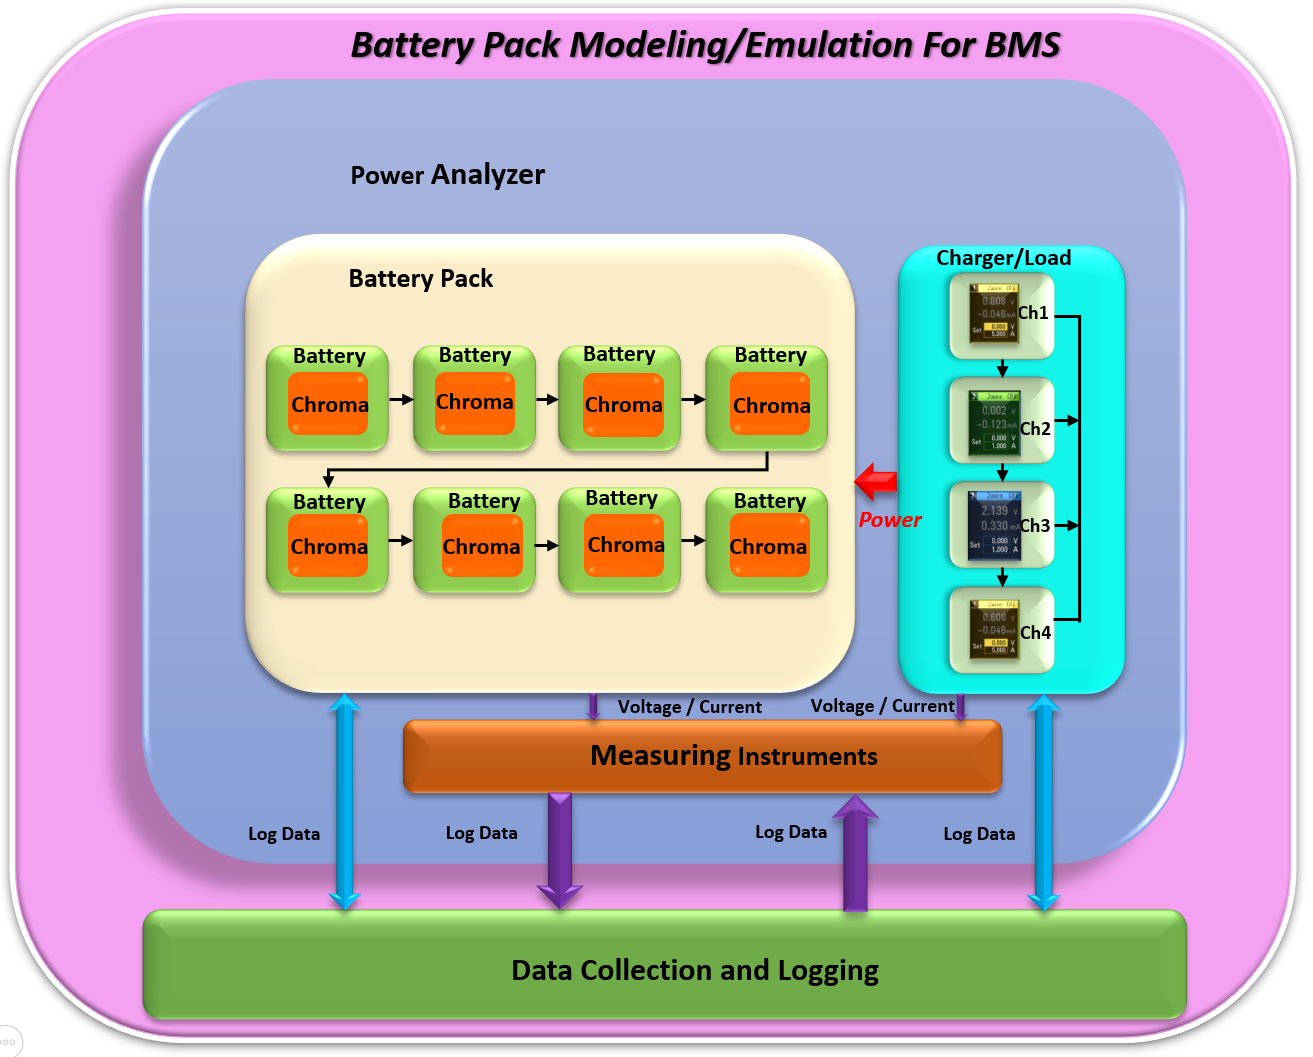
\includegraphics[width=0.9\textwidth]{Chap06/Figures/Battery_Pack_modeling_Architec.PNG}
	\caption{Architecture of the Battery Pack Modeling/Emulation For BMS}
	\label{fig:Battery_Pack_modeling_Architec}
\end{figure}

\subsection{Fundamental Instruments For Battery Emulation }

Figure \ref{fig:Battery_Pack_modeling_Architec} shows the architecture of the Battery modeling and the emulation, for the external view the architecture looks very clumsy and dusky, but I have followed the modular approach in this architecture to extend the model to a one-time constant or two-time constant even three. The proposed architecture can handle multiple current sourcing, sinking, and measuring instruments without disturbing the overall system. Before diving into the architecture and modular approach, it is good to understand what kind of instruments can be used. And their specifications for the BMS applications. The following section can give brief information on the instruments and their configurations.

\subsubsection{Chroma :}
\begin{figure}[h]
	\centering
	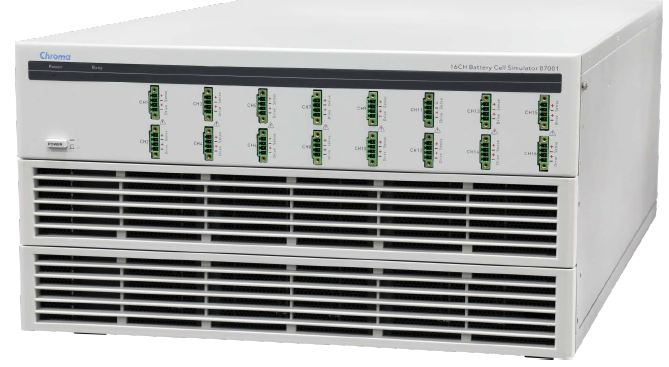
\includegraphics[width=0.5\textwidth]{Chap06/Figures/Chroma.PNG}
	\caption{16CH Battery Cell Simulator 87001}
	\label{fig:Chroma}
\end{figure}
The 87001 16CH Battery Cell Simulator can simulate the cell to perform charge and discharge behavior for BMS testing. It can simulate up to 480 battery cells in series with voltage and current measurement functions. It can receive IPC's commands in real-time, store the measured values temporarily and return them to the IPC \cite{Chroma_UserManual}.Chroma has two communication one through the ethernet and CAN bus, for facilitating the modular and easy communication I preferred ethernet for this particular project, we can also use the can bus when we test the emulator with the real-time vehicle setup. Figure \ref{fig:Chroma} shows the 16CH chroma which I have used in the lab.

\paragraph{Sepcifications of the Chroma :}

\begin{itemize}
    \item This simulator has built a DC Power Supply with 1Φ110~220V±10$\%$VLN input power.
    \item Each unit has 16 channels output that can set parameters, start and end time respectively.
    \item The channel can be a constant voltage source with a constant current function.
    \item Maximum 30 sets of 87001 simulators can be connected in series for use, and able to simulate the battery cell voltage of a 480-cell battery pack (2000V/4.2V) in series.
    \item High-precision output and measurement that are used in laboratories for testing product specifications and characteristics.
    \item No display panel and operation buttons but using LED lights to indicate the standalone unit status.
    \item Each channel has 2 current ranges (2 Current: (-5A~+5A, -0.5A~+0.5A) ).
    \item The operating interface uses the internet to give commands, control output measurement and read data via an external PC. The communication interface is Ethernet with SCPI protocol specification.
    \item Channels can be connected in series/parallel across a standalone unit with up to two batteries connected in parallel.
    \item Noise < 60db (output terminal 5V/5A/16CH)
    \item \textbf{Auto Range Select }
            \begin{itemize}
                \item The CC automatically switches to the proper range according to the set current.
                \item The CV automatically switches to the mapping range according to the upper limit current.
            \end{itemize} 
    \item \textbf{Current Range Select }
            \begin{itemize}
                \item When 5A is in use, performing CC charge for 500uA may have a bigger error.
                \item When 500mA is in use, performing CC charge for 5A will prompt a warning and stop execution.
            \end{itemize}

    \item \textbf{Data Transmission :} The data transmission interval is 10ms * paralleled unit no. The minimum data transmission interval is Δ10ms for one unit and Δ20ms for two units, and so forth.
    
\end{itemize}

\paragraph{Programing the Chroma:}

For Programing the Chroma I took the help of the pyvisa library, which can use to interface with instruments using different protocols. The first setup is the NI (National Instrument) driver in PC to identify the instrument (install NI Max application in PC), through the NI driver, pyvisa can communicate through the VISA virtual port. The piece of code shows how to configure the visa port for the chroma(or any battery emulator commands that are more generalized).

% \lstinputlisting[language=python]{Chap06/Code/Chroma.py}
\begin{lstlisting}[language=Python, caption=VISA parameters set for Chroma]
    #VISA commands for the Chroma
    set_visa_attribute(pyvisa.constants.VI_ATTR_MAX_QUEUE_LENGTH, 50)
    set_visa_attribute(pyvisa.constants.VI_ATTR_TMO_VALUE, 2000) #Time Out Value 
    set_visa_attribute(pyvisa.constants.VI_ATTR_TERMCHAR_EN, 
                        pyvisa.constants.VI_TRUE)
    set_visa_attribute(pyvisa.constants.VI_ATTR_TERMCHAR, 0xA) 
    set_visa_attribute(pyvisa.constants.VI_ATTR_SEND_END_EN, 
                       pyvisa.constants.VI_TRUE) 
    
    set_visa_attribute(pyvisa.constants.VI_ATTR_SUPPRESS_END_EN, 
                       pyvisa.constants.VI_TRUE)
    set_visa_attribute(pyvisa.constants.VI_ATTR_FILE_APPEND_EN, 
                       pyvisa.constants.VI_FALSE) 
    set_visa_attribute(pyvisa.constants.VI_ATTR_IO_PROT, 1) 
    set_visa_attribute(pyvisa.constants.VI_ATTR_TCPIP_NODELAY, 
                       pyvisa.constants.VI_TRUE) 
    set_visa_attribute(pyvisa.constants.VI_ATTR_TCPIP_KEEPALIVE, 
                       pyvisa.constants.VI_TRUE)
\end{lstlisting}

The following code explores the basic programming of the chroma for BMS application:

\begin{lstlisting}[language=Python, caption=Basic BMS Program for Chroma]
    #Basic Program for Chroma to configure the cells
    chroma.query('*IDN?\n') # identify the instrument
    #Query the output sampling time
    chroma.query('SIM:CONF:SAMP:TIME?\n') 

    #number of BMS(each Chroma is One BMS) are parallel
    chroma.write(f'SYST:SLAVE:PARA {self.noOfBMS}\n')
    chroma.write(f'SYST:SLAVE:SCAN {self.noOfBMS}\n')

    #Chroma Status commands
    chroma.query('SYSTem:FRAME:STATe? 0\n')
    chroma.query('SYST:FRAME:CHAN:STATe? 1\n')
    chroma.query('SYST:FRAME:CHAN:NUMB? 0\n')
    chroma.write('SIM:CONF:CHAN:ACT 65535\n')
    chroma.write('SIM:CONF:CLE\n'

    ''' BMS configurations '''
    #Number of the BMS 1
    chroma.write(f'SIM:CONF:BMS:NUMB {noOfBMS}\n')
    #No cells use in the BMS testing #1 BMS , #2 Cells 
    chroma.write(f'SIM:CONF:CELL:NUMB {noOfBMS},{noOfBMSCells}\n')
    #BMS 1, CellStart 1, Cellend 2, 
    # Cell parallel to the channel1 , # Current Range 2  - 5.0 A
    chroma.write(f'SIM:CONF:CELL:PARA {noOfBMS},{noOfBMS},
    {noOfBMStestingCells},{paralleBMSchannel},{cellCurrent_5A}\n') 

    ''' Output Parameters Set '''

    ''' # BMS start  1 ,# BMS end 1 ,#set the start cell 1, 
    # set the end cell 1, # set the cell voltage 4.0 ,
     # set the Current of the cell 0.5A '''

    chroma.write(f'SIM:PROG:CELL {noOfBMS},{noOfBMS},{cellNo},
    {cellNo},{cellVoltage},{cellCurrent5A}\n') 

    # Switch on all the cells immediately
    chroma.write('SIM:OUTP:IMM\n') 

    '''### check if there is any error 
    in the Chroma while setting the voltages 
    ### if there is no error enable
     all the cells outputs''' 

    time.sleep(10)
    # Check the configuration Error 
    self.chroma.query('SYST:ERR?\n')

    # Switch on all the cells
    self.chroma.write('SIM:OUTP ON \n')  
    time.sleep(1) # give some time to switch on the emulator 

\end{lstlisting}

% The above-attached code is just a basic code for the BMS application which can give a better idea about the basic chroma(Battery emulator) for more SCPI commands of the chroma follow the user manual\cite{Chroma_UserManual} and for the detailed class-based skeleton follow here %\href{}{here}.